\title{Dependent Types and Martin-L\"of Type Theory: An Introduction}
%% \title{Dependent Types and Type Theory: An Introduction}
\author{Carl Factora}
\date{\today}

\documentclass[12pt]{article}
% The following packages are needed because unicode
% is translated (using the next set of packages) to
% latex commands. You may need more packages if you
% use more unicode characters:
\usepackage{amssymb}
\usepackage{bbm}
\usepackage[greek,english]{babel}
% This handles the translation of unicode to latex:
\usepackage{ucs}
\usepackage[utf8x]{inputenc}
\usepackage{autofe}
\usepackage{tikz}
\usetikzlibrary{matrix}
\usetikzlibrary{arrows}

% Some characters that are not automatically defined
% (you figure out by the latex compilation errors you get),
% and you need to define:
\DeclareUnicodeCharacter{8988}{\ensuremath{\ulcorner}}
\DeclareUnicodeCharacter{8989}{\ensuremath{\urcorner}}
\DeclareUnicodeCharacter{8803}{\ensuremath{\overline{\equiv}}}
\DeclareUnicodeCharacter{120738}{\ensuremath{\Sigma}}
\DeclareUnicodeCharacter{955}{\ensuremath{\lambda}}
\DeclareUnicodeCharacter{2261}{\ensuremath{\equiv}}

% Add more as you need them (shouldn’t happen often).
% Using “\newenvironment” to redefine verbatim to
% be called “code” doesn’t always work properly. 
% You can more reliably use:
\usepackage{fancyvrb}

\DefineVerbatimEnvironment
  {code}{Verbatim}
  {} % Add fancy options here if you like.

\begin{document}
\maketitle

%% \begin{abstract}
%% \end{abstract}

\section{Introduction}
We present an introduction to dependent types and (Martin-L\"of) type theory.
At its core, type theory seeks to serve as a possible foundation of mathematics,
which itself is based on a different logical foundation. This proof-relevant
form of mathematics is the basis in which types can be used to model logical
propositions and is the core idea of type theory. As such, not only does type
theory have a viable application in mathematics but also in computer science,
providing for both a richer world of types and expressibility.

The study of type theory goes hand in hand with the study of dependent types,
which is  why we first take the time to do familiarize ourselves with them in
Section 2. We then continue with the foundational concepts of type theory of
Per Martin-L\"of \cite{}. In this section, while reading through the examples
we have provided, we recommend using a proof assistant, such as Agda. In our
examples, we refer to Agda notation. 

\section{Dependent Types}
In this section, we introduce the concept of dependent types and their role in
type theoretic systems. At their core, dependent types can be thought of simply
as an \textit{interplay of types and terms}. To understand this relationship,
it helps to think of the ways in which types and terms can \textit{depend} on
one another. Altogether, this results in four dependencies:

\begin{enumerate}
\item terms depending on terms
\item terms depending on types
\item types depending on types
\item types depending on terms
\end{enumerate}
These dependecies, however, should not be confused with an actual dependent
type. In fact, only (2) and (4) correspond to expressions that are typed
(necessarily) with a dependent type (we explain later why (1) and (3) are
not typed with dependent types).

What follows is a brief description of each form of dependency and the
corresponding \(\lambda\)-calculus that is associated with it. With this, we
introduce the (fully-dependent) system of the \textit{Calculus of Constructions}
(\(\lambda C\)) \cite{}. Here, the word \textit{fully} signifies that \(\lambda C\)
features all four forms of dependency mentioned above.

\subsection*{Simply-Typed (STLC)}
\subsubsection*{Role: Base System}
The STLC is not a dependently typed system. In fact, the term {\em dependent type}
is drawn in constrast with the term {\em simple type}, where the STLC derives
its namesake. A simple type is either a {\em primitive type}, which is the set
of all types ``pre-defined'' (e.g. lists, numbers, booleans), or a
{\em function type} between other simple types. Thus, simple types have the
following grammar:
\begin{center}
\begin{minipage}{0.5\textwidth}
\begin{code}
t || t → t
\end{code}
\end{minipage}
\end{center}
The terms of the STLC are the terms of the \textit{untyped \(\lambda\)-calculus},
with the exception of terms that use \textit{self-application} (i.e., Y
combinator, Omega, etc.). An example term, annotated with its type, is generally
written as follows:
\begin{center}
\begin{minipage}{0.5\textwidth}
\begin{code}
example : ℕ → ℕ
example = λ (z : ℕ) → z
\end{code}
\end{minipage}
\end{center}
Or, equivalently,
\begin{center}
\begin{minipage}{0.5\textwidth}
\begin{code}
example = λ z → z
\end{code}
\end{minipage}
\end{center}
whenever the type of the argument (viz. {\tt z}) is easily inferable.

This leaves the STLC rather small and limited but has the benefit of removing
all \textit{infinite} calculations from the system \cite{}. Thus, the STLC is
not \textit{Turing complete} and is thus the appropriate foundation for
deriving a type theoretic system. This is because the STLC lends itself quite
seamlessly as component of a larger, more expressive system. This flexibility
is what we exploit to derive \(\lambda C\). To do this, we first extend the STLC
with more expressive types through simple extentions on its grammar for simple
types.

%% as the only form of dependency
%% present in the STLC is (1), terms depending on terms (i.e. {\em term level}
%% \(\lambda\)-abstraction).

The key difference between the STLC and \(\lambda C\) are the places in which
terms and types are allowed to be. In the STLC, terms and types are entirely
seperate entities in that terms only exist on {\em term level} and types
on {\em type level}. Thus, as we mentioned earlier, this puts a constraint
on the system to only allow \(\lambda\)-abstraction to happen at term level
(viz. definition of simple type). For example, the \textit{constant function}
over types \(\mathbb{N}\) and \(\mathbb{B}\) in the STLC is defined:
\begin{center}
\begin{minipage}{0.5\textwidth}
\begin{code}
const : ℕ → 𝔹 → ℕ
const = λ n b → n
\end{code}
\end{minipage}
\end{center}
Given that {\tt const} is of type {\tt ℕ → 𝔹 → ℕ}, the term that inhabits this
type is {\tt λ n b → n}. In this example, we can see that terms and types are
treated differently and are only related in terms of {\em inhabitance}. This
relation is reason for the limited expressivity of the STLC and is also the
method in which the STLC can be extended into \(\lambda C\).

\subsection*{Second-Order (\(\lambda2\))}
\subsubsection*{Role: Addition of polymorphic functions}

Another name for \(\lambda2\) is System F \cite{}. For our purposes, we treat
\(\lambda2\) as simply an extension of the STLC. This system is adds
{\em polymorphic} terms to the STLC (viz. Dependency (2)). For example,
let's take the definition of {\tt const} above and change it to define
{\tt polyConst}:
\begin{center}
\begin{minipage}{0.5\textwidth}
\begin{code}
polyConst : (A B : Set) → A → B → A
polyConst A B = λ a b → a
-- Works for any type A and B
\end{code}
\end{minipage}
\end{center}

Unlike {\tt const}, {\tt polyConst} takes four arguments, where the first two
are types. These two types (viz {\tt A} and {\tt B}) are the corresponding
types of the third and fourth arguments of {\tt polyConst}. To clarify, we can
instantiate {\tt polyConst} with \(\mathbb{N}\) and \(\mathbb{B}\) resulting
in a function of type {\tt ℕ → 𝔹 → ℕ}, giving us

$${\tt const} = {\tt polyConst(ℕ,𝔹)}.$$
Thus, adding polymorphism to the STLC has the effect of extending the notion
of type and term. With \(\lambda2\), we are now allowed to pass types as arguments
at term level (viz. we pass the actual types \(\mathbb{N}\) and \(\mathbb{B}\)).
It is, however, necessary to constrain this expressivity with a more expressive
type (e.g. {\tt (x : A) → ...}). Types that appear in this fashion are
called \(\Pi\)-types. Taking the grammar for simple types, we can add \(\Pi\)-types,
resulting in the grammar for types ({\tt t}) in \(\lambda2\):

\begin{center}
\begin{minipage}{0.5\textwidth}
\begin{code}
t || t → t || ∀ (x : Set) → t
\end{code}


\end{minipage}
\begin{minipage}{0.65\textwidth}
\begin{small}
In general, the \(\forall\) symbol is used to express \(\Pi\)-types
\end{small}
\end{minipage}
\end{center}

Briefly, \(\Pi\)-types are a form of dependent type that are inhabited by
polymorphic functions. In cases like {\tt polyConst}, \(\Pi\)-types are
necessary to signify the treament of a polymorphic function and to prevent
the appearance of free variables within type expressions. For example,
if we had typed {\tt polyConst} as {\tt A → B → A}, then {\tt A} and {\tt B} are
free variables in that they, by themselves, have no {\em meaning}. This is why
{\tt polyConst} is first passed two types to instantiate the meanings of {\tt A}
and {\tt B}. In a sense, a \(\Pi\)-type binds values for types just as
\(\lambda\)-abstraction binds values for terms.

\(\Pi\)-types are actually significantly more expressive than the ones in
\(\lambda2\). In \(\lambda2\), they are constrained to be only parameterized
over other types (e.g. {\tt Set} in {\tt ∀ (x : Set) → t}). In a later system, we
allow \(\Pi\)-types to be parameterized over terms (e.g. {\tt ∀ (x : t) → t}).

So far, we've seen how terms can depend on other terms (STLC) and how terms can
depend on types (term level polymoprhism). In the following system, we introduce
a small, yet important dependency: types depending on types.

\subsection*{Higher-order (\(\lambda\underline{\omega}\))}
\subsubsection*{Role: Addition of type constructors}

To clarify, \(\lambda\underline{\omega}\) is generally not a standalone system,
instead, it is generally treated as an ``add-on'' system. Later, we model the
relationship of each system to \(\lambda C\). For the sake of time, we treat
\(\lambda\underline{\omega}\) as an extension of \(\lambda2\), giving us the
following transition:

\begin{center}
\begin{minipage}{0.4\textwidth}
STLC \(\rightarrow\) \(\lambda2\) \(\rightarrow\) (+\(\lambda\underline{\omega}\)) \(\rightarrow\) \(\lambda\omega\)
\end{minipage}
\end{center}

Thus, the system we are introducing is \(\lambda\omega\), which, unlike
\(\lambda\underline{\omega}\), features a more diverse grammar of types (i.e.,
\(\lambda\underline{\omega}\) does not have \(\Pi\)-types). Given its \(\lambda2\)
component, another name for this system is System F\(\omega\). Before we introduce
the new grammar for types, we first introduce the concept of {\em levels}.

We are already familiar with the first two levels, terms and types, which, from
the STLC, are related in terms of inhabitance. To introduce the third level and
onward, we must also provide the type of types. For our purposes, we assume an
infinite universe of types, as is common practice in deriving type theoretic
systems to avoid certain paradoxes \cite{}. For example, let's first assume that
natural numbers are primitive within our system. We then have the following for
the natural number 42:

\begin{center}
\begin{minipage}{0.4\textwidth}
\begin{code}
42 : ℕ : Set : Set₁ ...
\end{code}
\end{minipage}
\end{center}

We read the above example as: 42 is of type \(\mathbb{N}\) which is of type
{\tt Set} which of type {\tt Set₁} and so on. There is, however, an important
distinction for the first two levels: 42 is NOT of type {\tt Set}, while
\(\mathbb{N}\) is both of type {\tt Set}, {\tt Set₁} and onwards. Terms are
therefore treated uniquely, since they only exist as elements of types.

We can now revise the definition of types ({\tt t}) to include all instances of
{\tt Set} in our infinite universe. We notate this as {\tt Set} below:

\begin{center}
\begin{minipage}{0.65\textwidth}
\begin{code}
t || t → t || ∀ (x : Set) → t || Set
\end{code}
\end{minipage}
\end{center}

The curious effect of doing this allows us to construct expressions of type
{\tt t → t}, where either {\tt t} can have subexpressions containing {\tt Set}.
Let's take the familiar definition of the list data structure:

\begin{center}
\begin{minipage}{0.65\textwidth}
\begin{code}
data List (A : Set) : Set where
  Nil  : List A
  _::_ : A → List A → List A
\end{code}
\end{minipage}
\end{center}

We discuss {\tt List} more in depth in a later section. For now, we simply ask
{\em what is the type of {\tt List}?} To answer this question, we can simply
look at the first line of the definition above (viz. {\tt List (A : Set) : Set}).
From this line, we can see that {\tt List} is a type parameterized over any type
{\tt A}. Another way to think about this statement is to think of {\tt List} as
a form of polymorphic function of type {\tt Set → Set}, as is similar with other
{\em parameterized types}. Unlike like {\tt const} or {\tt polyConst}, this
function can only be applied at type level (thus the name {\em type constructor}).
This is to insure that we cannot write type expressions that fail to instantiate
{\tt List} (e.g. {\tt List → A} v. {\tt List A → A}).

From this we can see that the addition of {\tt Set} into our grammar of
types has great effect on the expressivity of our system. There is only one
other extension necessary to consider our system fully-dependently typed, which,
similar to our treatment of \(\lambda\underline{\omega}\) is also deceptively
simple.

\subsection*{Predicates (\(\lambda P\))}
\subsubsection*{Role: Encoding of Propositional logic}

To review, if we compile all the previously mentioned systems above, we have
the system \(\lambda\omega\) (System F\(\omega\)). Our final addition, the
system of \(\lambda P\), allows us to construct {\em type families} which are
types themselves and are meant to directly correspond to propositions in
higher-order logic.

Let's take a simple example. Let's define a proposition {\tt isEven} that takes
a natural number. Another way to say this is that {\tt isEven} is a predicate
over natural numbers. When writing propositions, we write them as their equivalent
type definition (similar to {\tt List}). Consequently, the proposition
{\tt isEven} is an example of a dependent type, since its {\em meaning} depends
on the natural number passed to it (types depending on terms).

\begin{center}
\begin{minipage}{0.7\textwidth}
\begin{code}
data _isEven : ℕ → Set where
  ZEven : 0 isEven
  NEven : ∀ n → n isEven → (Suc (Suc n)) isEven
\end{code}
\end{minipage}
\end{center}

Here, we've defined two ways in which {\tt n isEven} for all natural numbers
({\tt n}) can be proven. Returning to the idea of proof-relevant mathematics,
we do this by use of its two type constructors {\tt ZEven} and {\tt NEven},
corresponding to the two constructors of \(\mathbb{N}\). {\tt ZEven} is the
proof that 0 is an even number. {\tt NEven} then defines the property that if
a given natural number ({\tt n}) is even (viz. {\tt n isEven}), then {\tt n + 2}
is even (viz. {\tt (Suc (Suc n)) isEven}). To clarify how this type can be used,
let's prove that 4 is even. We start by providing the appropriate type definition
and also providing a name for our proof (viz. {\tt 4isEven}):
\begin{center}
\begin{minipage}{0.5\textwidth}
\begin{code}
4isEven : 4 isEven
\end{code}
\end{minipage}
\end{center}
From the definition of {\tt isEven}, we know that to prove 4 is even, we must
know that 2 is even. Consequently, to prove 2 is even, we must know that 0 is
even. Fortunately, we have a proof that 0 is even: {\tt ZEven}. Thus, the proof
that 2 is even is {\tt NEven 0 ZEven}, and finally the proof that 4 is even is:
\begin{center}
\begin{minipage}{0.5\textwidth}
\begin{code}
4isEven : 4 isEven
4isEven = NEven 2 (NEven 0 ZEven)
\end{code}
\end{minipage}
\end{center}

This method of proof is adopted from {\em Intuitionistic Logic} \cite{}. In
this form of logic, ``truth'' corresponds to the idea of {\em type inhabitability}.
This makes sense since we use types to correspond to logical propositions
(e.g. {\tt isEven}). ``Falsity'' then naturally corresponds to the un-inhabitability
of a given type. This can be seen if we try to prove that 5 is even using
{\tt isEven}. The proof seems to get ``stuck'' at trying to prove that 1 is even.

While it might seem intuitive and more effective to instead try to prove that 5
is {\em not} even, this, however, also doesn't work. This is due to the
treatment of negation in Intuitionistic Logic. To prove that 5 is not even is
to prove that \(\neg (5\) {\tt isEven}), which is equivalent to constructing a
function of type:
\begin{center}
\begin{minipage}{0.2\textwidth}
\begin{code}
5 isEven → ⊥
\end{code}
\end{minipage}
\end{center}
That is, given a proof that {\tt 5 isEven}, construct \(\perp\), the empty type.
This is not possible since we cannot ever construct a proof that 5 is even. We
discuss the empty type later in Section 3.

\subsection*{Calculus of Constructions and Remarks}
To conclude our discussion over dependent types, we present the final grammar for
types after extending \(\lambda\omega\) with \(\lambda P\):
\begin{center}
\begin{minipage}{0.5\textwidth}
\begin{code}
t || t → t || ∀ (x : t) → t || Set
\end{code}
\end{minipage}
\end{center}
It should come with no surprise that the change is minor. We simply have lifted
the restriction on \(\Pi\)-types and allowed them to be parameterized over both
terms and types.

In the process of introducing dependent types, we have shown the necessary
changes and extensions on the STLC to achieve the expressivity necessary to
function as a foundation for mathematics. To clarify this process and to show
the relationship between each of the systems we have previously mentioned, we
include a diagram of the {\em Lambda Cube} \cite{}:
\begin{center}
  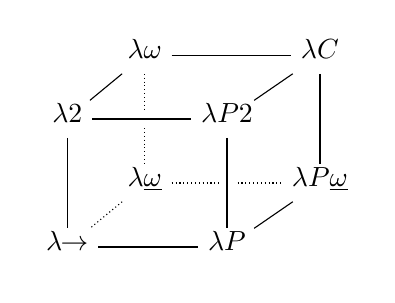
\begin{tikzpicture}[
      back line/.style={densely dotted},
      cross line/.style={preaction={draw=white, -,
          line width=6pt}}]
    \matrix (m) [matrix of math nodes,
      row sep=1em, column sep=.75em,
      text height=1ex,
      text depth=0.5ex]{
      & \lambda\omega & & \lambda C \\
      \lambda 2 & & \lambda P2 \\
      & \lambda\underline\omega & & \lambda P\underline\omega \\
      \lambda\!\!\rightarrow  & & \lambda P \\
    };
    \path[-]
    (m-1-2) edge (m-1-4)
    edge (m-2-1)
    edge [back line] (m-3-2)
    (m-1-4) edge (m-3-4)
    edge (m-2-3)
    (m-2-1) edge [cross line] (m-2-3)
    edge (m-4-1)
    (m-3-2) edge [back line] (m-3-4)
    edge [back line] (m-4-1)
    (m-4-1) edge (m-4-3)
    (m-3-4) edge (m-4-3)
    (m-2-3) edge [cross line] (m-4-3);
  \end{tikzpicture}
\end{center}
Reading the cube requires us to start on the edge marked \(\lambda\!\!\rightarrow\),
which corresponds to the STLC, the base system. From here, we can either move
inwards, upwards, or rightwards, which corresponds to the extension to the
other systems marked on the respective edges. Using only these three movements,
we eventually reach \(\lambda C\), leaving it in the {\em most powerful}
position on the cube.

\section{Martin-L\"of Type Theory}
%% Curry-Howard?
In this section, we introduce the foundational concepts of Martin-L\"of Type
Theory \cite{}. We discuss recursion, induction, and as well several primitive type
encodings (from propositional logic).

\subsection*{Principles}
Recursion and induction are one of the powerful tools available in a
fully-dependently typed system. Recursion and induction principles can be
thought of as specialized functions to behave on elements of a given type.
If we use recursion and induction principles to define functions and proofs,
we are guaranteed both termination and totality. This is because, in general,
recursion and induction principles are defined under certain known intuitions
(which is why they are sometimes considered axioms) on the given type that
they are meant to act on.

These principles follow a certain pattern:
\begin{center}
\begin{minipage}{0.9\textwidth}
\begin{code}
recT : (C : Set) → C₀ ... → T → C
indT : (C : T → Set) → (C₀ : ...) ... → (t : T) → C t
\end{code}
\end{minipage}

\begin{minipage}{0.7\textwidth}
\begin{small}
The recursion and induction principles for some type {\tt T}.
\end{small}
\end{minipage}
\end{center}
The first argument given to these principles is sometimes called the {\em motive}.
This simply means that {\tt C} is the type from which we will return a element
from. For recursion principles, this means the given output of the function we
are defining, and for induction principles, this can be read as the proposition
we are trying to prove. The terms that follow (viz. {\tt C₀}) correspond to the
constructor(s) of the given type, which is how these principles guarantee
totality. Finally, both principles take a term of the type that are acting on
(viz. {\tt T} and {\tt (t : T)}). The only difference is that the induction
principle introduces a type family, as opposed to a non-parameterized type in the
recursion principle. We discuss this in Section 4.

In this section, we discuss the recursion and induction principles, {\tt rec}
and {\tt ind}, for each {\em primitive type}: \(\perp\), \(\top\), +,
\(\times\), and \(\Sigma\). The symbols + and \(\times\) signify disjunction
and conjunction and, thus, should not be confused with addition and
multiplication. For the latter, we use the names {\tt plus} and {\tt times}.

\subsection*{Primitive Type Encodings}
%% Bottom, Top, Disjunction, Conjunction, Sigma
We start with \(\perp\), the empty type. Since there no ways to construct
an element of the empty type, the encoding is rather simple:
\begin{center}
\begin{minipage}{0.9\textwidth}
\begin{code}
data ⊥ : Set where

rec⊥ : (C : Set) → ⊥ → C
rec⊥ C ()

ind⊥ : (C : ⊥ → Set) → (z : ⊥) → C z
ind⊥ C ()

prop : {A : Set} → ⊥ → A
prop {A} perp = rec⊥ A perp

prop' : {A : ⊥ → Set} → (x : ⊥) → A x
prop' {A} perp = ind⊥ A perp
\end{code}
\end{minipage}
\end{center}
The behavior of the empty type is meant to model {\it ex-falso} (i.e., from
absurdity comes anything we like). In general, we use the empty type when
writing proofs containing negated expressions.

To clarify our discussion about the empty type, we include a proof of:
$$\neg\neg\neg A\rightarrow\neg A$$
Here, we define negation, \(\neg\), to be a function, such that:
\begin{center}
\begin{minipage}{0.9\textwidth}
\begin{code}
¬ : Set → Set
¬ A = A → ⊥

prop₀ : {A : Set} → ¬ (¬ (¬ A)) → ¬ A
prop₀ ¬¬¬a a = ?
\end{code}
\end{minipage}
\end{center}
Now, we solve for {\tt ?}. Looking at the type expression of {\tt prop₀},
we know we have an expression of type \(\neg\neg\neg A\) and also an
expression of type \(A\). To clarify, we can rewrite the type expression
after desugaring \(\neg A\):
$$\neg\neg\neg A\rightarrow A\rightarrow\perp$$
Now, to construct an element of type \(\neg A\) from an element of type
\(\neg\neg\neg A\), we can use the definition of \(\neg\):
$$(\neg\neg A\rightarrow\perp)\rightarrow A\rightarrow\perp$$
$$((\neg A\rightarrow\perp)\rightarrow\perp)\rightarrow A\rightarrow\perp$$
$$(((A\rightarrow\perp)\rightarrow\perp)\rightarrow\perp)\rightarrow A\rightarrow\perp$$
Thus, we know we must apply our expression \(\neg\neg\neg A\) to a function
of type \(\neg\neg A\) and so on, such that:
\begin{center}
\begin{minipage}{0.9\textwidth}
\begin{code}
prop₀ : {A : Set} → ¬ (¬ (¬ A)) → ¬ A
prop₀ ¬¬¬a a = ¬¬¬a (λ ¬a → ¬a a)
\end{code}
\end{minipage}
\end{center}
Or equivalently:
\begin{center}
\begin{minipage}{0.9\textwidth}
\begin{code}
prop₀ ¬¬¬a a = rec⊥ ⊥ (¬¬¬a (λ ¬a → ¬a a))
\end{code}
\end{minipage}
\end{center}

Next, we introduce the type \(\top\), which contains exactly one element,
{\tt *}:
\begin{center}
\begin{minipage}{0.9\textwidth}
\begin{code}
data ⊤ : Set where
  * : ⊤

rec⊤ : (C : Set) → C → ⊤ → C
rec⊤ C c * = c

ind⊤ : (C : ⊤ → Set) → C * → (x : ⊤) → C x
ind⊤ C c * = c
\end{code}
\end{minipage}
\end{center}
Similar to \(\perp\), \(\top\) is simple and is rather uninteresting by itself.
There are, however, some trivial yet interesting proofs that involve the two.
The first of these we also introduce a special kind of proof: {\it uniqueness
of identity} (UIP) \cite{}. In this proof, we set out to determine and classify
the identity of every element within a given type. For example, for \(\top\), we
should be able to prove:
$$\forall (x : \top) \rightarrow x ≡ *$$
That is, for every element of type \(\top\), that element is equivalent to {\tt *}.
This second expression, {\it x ≡} {\tt *}, is an example of an {\it identity type},
which we describe later on in this section. For now, we simply say that the
sole constructor for the identity type is {\it refl x}, for all x.

Now, to prove the above proposition, we can use the induction principle for
\(\top\), since the proposition we are trying to prove concerns all elements
of \(\top\):
\begin{center}
\begin{minipage}{0.9\textwidth}
\begin{code}
uip⊤ : (x : ⊤) → x ≡ *
uip⊤ x = ind⊤ (λ top → top ≡ *) (refl *) x
--uip⊤ * = refl *
\end{code}
\end{minipage}
\end{center}
Here, we have taken our motive to be the expression {\tt (λ top → top ≡ *)},
which essentially repeats the information already given by our type expression.
The second element, {\tt refl *}, is a proof that our motive holds in the event
{\tt top} is {\tt *}, which is of type {\tt * ≡ *}. The last element {\tt x} is
the expression initially passed to our proof of type \(\top\). Equivalently, we
could have also written our proof as the third line above. This form of proof
uses pattern matching and essentially asserts that the only element in \(\top\)
is {\tt *}, which greatly simplifies our proof. Both methods of proof are
correct, but, in general, using pattern matching is only safe when the values of
proof expressions are not dependent one another (i.e., their values don't change
depending on which expression we apply pattern matching to).

Before we can do more proofs, we first introduce the disjunction type, +: 
\begin{center}
\begin{minipage}{0.9\textwidth}
\begin{code}
data _+_ (A B : Set) : Set where
  inl : A → A + B
  inr : B → A + B

rec+ : {A B : Set} (C : Set) → (A → C) → (B → C) →
       A + B → C
rec+ C f _ (inl a) = f a
rec+ C _ f (inr b) = f b

ind+ : {A B : Set} (C : A + B → Set) →
       (∀ (x : A) → C (inl x)) →
       (∀ (x : B) → C (inr x)) →
       (x : A + B) → C x
ind+ C f _ (inl a) = f a
ind+ C _ f (inr b) = f b
\end{code}
\end{minipage}
\end{center}
It might come as surprise as to why the symbol for addition is generally used
for the disjunction type. This is because another name for + is a {\it union type}.
This type is parameterized over two other types, {\tt A} and {\tt B}, and
creates a union between them in that every expression of type {\tt A + B} is
either {\tt inl a}, where {\tt a : A}, or {\tt inr b}, where {\tt b : B}.

\section{Example Types and Sample Proofs}
In this section, we present the type of Booleans, Natural numbers, Lists,
and the identity type. To further understand these types, we also include
a brief description of the different forms of equality, namely definitional,
judgmental and propositional. In type theory, the specific differences
between the three are generally misunderstood but are important in understanding
basic type theoretic proof methods, which we also go into some detail in
this section with several examples.

\subsection*{Equality}
%% talk about definitional equality, judgmental equality, prop equality

\subsection*{Booleans}
\begin{center}
\begin{minipage}{0.9\textwidth}
\begin{code}
data 𝔹 : Set where
  True  : 𝔹
  False : 𝔹

rec𝔹 : (C : Set) → C → C → 𝔹 → C
rec𝔹 C t f True = t
rec𝔹 C t f False = f

ind𝔹 : (C : 𝔹 → Set) → C True → C False → (x : 𝔹) → C x
ind𝔹 C t f True = t
ind𝔹 C t f False = f
\end{code}
\end{minipage}
\end{center}
%% proof: 1 + 1 = 2

\subsection*{Natural Numbers}
\begin{center}
\begin{minipage}{0.9\textwidth}
\begin{code}
data ℕ : Set where
  0 : ℕ
  suc : ℕ → ℕ

recℕ : (C : Set) → C → (ℕ → C → C) → ℕ → C
recℕ C c _ 0 = c
recℕ C c f (suc n) = f n (recℕ C c f n) 

indℕ : (C : ℕ → Set) → C 0 →
       (∀ (x : ℕ) → C x → C (suc x)) →
       (x : ℕ) → C x
indℕ C c _ 0 = c
indℕ C c f (suc n) = f n (indℕ C c f n)
\end{code}
\end{minipage}
\end{center}

\subsection*{List/Orderings}
\begin{center}
\begin{minipage}{0.9\textwidth}
\begin{code}
data List (A : Set) : Set where
  Nil  : List A
  _::_ : A → List A → List A

recList : {A : Set} → (C : Set) → C →
          (A → List A → C → C) → List A → C
recList C c f Nil = c
recList C c f (x :: xs) = f x xs (recList C c f xs)

indList : {A : Set} → (C : List A → Set) → C Nil →
          (∀ (x : A) → (xs : List A) → C xs → C (x :: xs)) →
          (xs : List A) → C xs
indList C c f Nil = c
indList C c f (x :: xs) = f x xs (indList C c f xs)
\end{code}
\end{minipage}
\end{center}

\subsection*{Identity Types}
%% say something that this is the HoTT version of identity
%% possibly also point out that the discrepancy between the two
\begin{center}
\begin{minipage}{0.9\textwidth}
\begin{code}
infix  4  _≡_
data _≡_ {ℓ} {A : Set ℓ} : (a b : A) → Set ℓ where
  refl : (a : A) → (a ≡ a)

-- "PROPOSITIONAL EQUALITY"
-- For a proposition, C, on a proof of x ≡ y for
-- any x and y, if we can show that it holds for
-- (refl x), then C holds for all proofs, p : x ≡ y.
J : {A : Set} (C : {x y : A} → x ≡ y → Set) →
    (∀ (x : A) → C (refl x)) →
    {x y : A} (p : x ≡ y) → C p
J C c (refl x) = c x

-- "STRICT EQUALITY"
-- For a proposition, C, on a reflexive equality (x ≡ x),
-- for any x, if we can show that it holds for (refl x), then
-- C holds for all other reflexive equalities p : x ≡ x.
K : {A : Set} (C : {x : A} → x ≡ x → Set) →
    (∀ (x : A) → C (refl x)) →
    {x : A} (p : x ≡ x) → C p
K C c (refl x) = c x

rec≡ : {A : Set} {x y : A} (C : A → Set) →
       (p : x ≡ y) → C x → C y
rec≡ {A} {x} {y} C = 
  J (λ {x} {y} _ → C x → C y)
    (λ x → λ z → z)
    {x} {y} 
\end{code}
\end{minipage}
\end{center}

\section{Discussion}
Say a few things about the paper.

\subsection*{Extension to Homotopy Type Theory}

\end{document}
